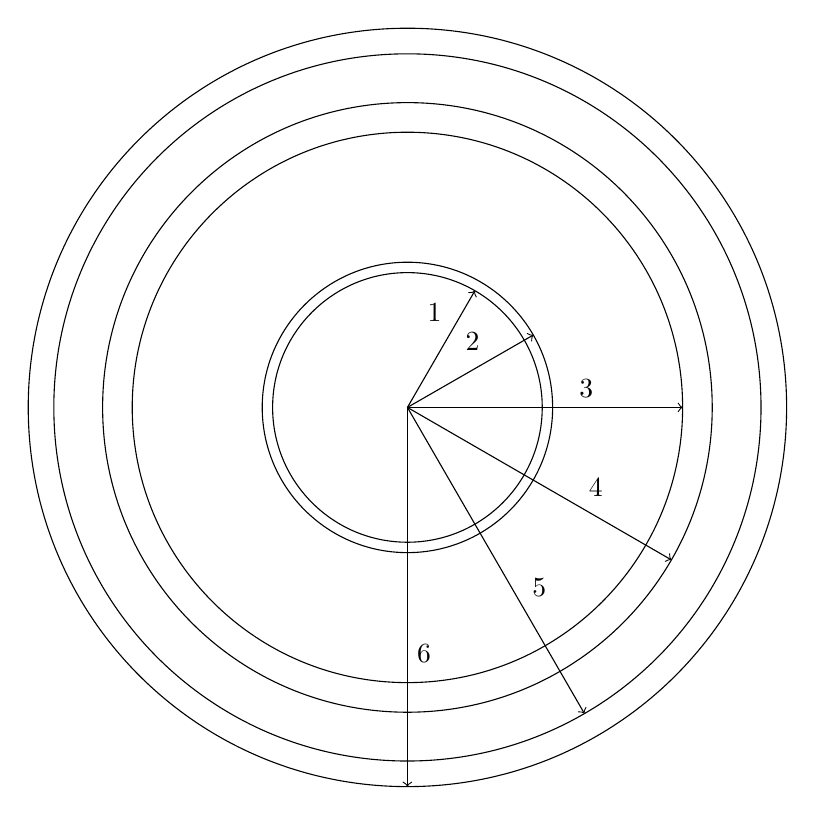
\begin{tikzpicture}[scale=8,auto]
        \draw (0,0) circle (0.214);
      \draw[->] (0,0) -- node[pos=0.65] {1} (0.107,0.185);
      \draw (0,0) circle (0.23051);
      \draw[->] (0,0) -- node[pos=0.65] {2} (0.2,0.115);
      \draw (0,0) circle (0.43688);
      \draw[->] (0,0) -- node[pos=0.65] {3} (0.437,0.0);
      \draw (0,0) circle (0.48387);
      \draw[->] (0,0) -- node[pos=0.65] {4} (0.419,-0.242);
      \draw (0,0) circle (0.56134);
      \draw[->] (0,0) -- node[pos=0.65] {5} (0.281,-0.486);
      \draw (0,0) circle (0.60198);
      \draw[->] (0,0) -- node[pos=0.65] {6} (0.0,-0.602);

      \end{tikzpicture}
      \begin{tikzpicture}
       \matrix [matrix of nodes]
      {
          Arrow & Radius (cm) & Material & \numrefheader \\
        1 & 0.21400 & \node[hyperlink node=mat_air]{Air}; & \ref{num:BPinnercladIR}\\ 
        2 & 0.23051 & \node[hyperlink node=mat_SS304]{SS304}; & \ref{num:BPinnercladOR}\\ 
        3 & 0.43688 & \node[hyperlink node=mat_helium]{Helium}; & \ref{num:BPoutercladIR}\\ 
        4 & 0.48387 & \node[hyperlink node=mat_SS304]{SS304}; & \ref{num:BPoutercladOR}\\ 
        5 & 0.56134 & \node[hyperlink node=mat_water]{Water}; & \ref{num:GTIRrad}\\ 
        6 & 0.60198 & \node[hyperlink node=mat_zirc]{Zircaloy}; & \ref{num:GTORrad}\\ 
      };
\end{tikzpicture}